\chapter{State of the Art} \label{chap:sota}

This chapter presents the fundamental concepts of underwater acoustics engineering for localization and positioning of aquatic autonomous vehicles. 

It starts by establishing the properties of the underwater acoustic channel, detailing on four main concepts. Then, a overview on underwater localization estimation is presented, addressing range estimation methods and position estimation techniques based on reference nodes. Thereafter the three most used types of underwater positioning systems are presented followed by some USBL commercial solutions and their specifications. Lastly, sensor configuration optimization methods are laid out.

\section{Underwater Acoustic Channel} \label{subsec: acoustic-channel}

Although satellite based navigation systems are the most commonly used for positioning and localization at the earth surface, the used radio signals are highly absorbed by the water and thus inappropriate for underwater localization and communication. Therefore, the state of the art solutions for long range localization and communications in the underwater environment rely on the propagation of acoustic signals.

The natural limitations of acoustic channels combined with the properties of an underwater environment, result in challenges and limitations in developing communication and localization systems \cite{survey-tech-chall}:

\begin{itemize}
	\item Long propagation delays make it unmanageable for underwater acoustic networks to employ some common data networks' mechanisms, such as acknowledgment-based protocols;
	
	\item Variable speed of the acoustic signals due to variations in temperature and density;
	
	\item Limited bandwidth, as the attenuation of acoustic waves increases with frequency;
	
	\item The path of acoustic signals is not a straight line since the sound waves are bent, due to sound speed variation along the water column, and reflected or blocked in many different surfaces, which may lead to the incorrect detection of the line-of-sight (LOS) signal;
	
	\item Attenuation and asymmetric signal-to-noise ratio, which arises from the fact that SNR depends on depth and frequency with complex behaviors that depend on the characteristics of the environment.
	
\end{itemize}

Underwater localization systems based on acoustic signals are the only effective way to work in distance ranges up to a few kilometers, as opposed to optical or radio-frequency based systems. However, these always unreliable characteristics lead to a significant degree of uncertainty as, in practice, it is impossible to know the exact speed and path of a sound wave along the path it actually travels.

This following subsections present a more detailed overview on various concepts that affect the underwater communication channels, such as the sound speed, multipath phenomena, the Doppler effect, signal attenuation and signal-to-noise ratio.

\subsection{Speed of Sound} \label{subsec: speed-sound}

The oceanic environment has a complex sound propagation model, as it comprises many variants.

Acoustic signals' propagation speed is mainly related to two factors: compressibility and density. The water density can be characterized by the temperature, salinity and pressure,which is associated with depth \cite{ocean-acoust}. Figure \ref{fig:spd-sound} exhibits a generic sound speed profile in relation to depth. The water surface is commonly a mixed layer that results in an approximately constant sound speed. After this layer, it suffers a significant decrease, usually reaching the lower tangible speed, which results from the variation of temperature that characterizes the thermocline layer. From that point forward, pressure is the greatest influencer on speed of sound, so it increases relatively proportionally to depth.

\begin{figure}[!htbp]
	\centering
	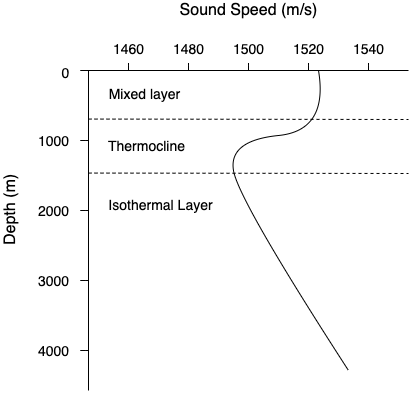
\includegraphics[width=0.6\textwidth]{figures/sound-profile}
	\caption{Generic sound speed profile}
	\label{fig:spd-sound}
\end{figure}

The empirical equation (\ref{eq:spd-sound}) \cite{ocean-acoust} is a simplified translation of the behavior of the sound speed \textit{c} in meters per second, with relation to the temperature \textit{T} in ºC, the salinity \textit{S} in parts per thousand and the depth \textit{z} in meters. 
\begin{eqnarray}
c = 1449.2 + 4.6T - 0.055T^2 + 0.00029T^3 + (1.34 - 0.01T)(S-35) + 0.016z 
\label{eq:spd-sound}
\end{eqnarray}

The varying sound speed throughout the water column causes the signals not to propagate in a straight line from a transmitter to a receiver. Therefore, when using positioning systems, such as USBL, the measurement of propagation times becomes inaccurate reflecting on lower system's localization precision.

\subsection{Multipath} \label{subsec:multipath}

Multipath occurs when signals suffer distortion that originate multiple propagation paths, leading to a change in their original characteristics. This phenomenon is originated by diverse factors that cause distortion in the underwater channels, typically affecting the water composition, such as temperature and depth. The signal distortions caused by multipath include signal fading, which is usually modeled by Rayleigh fading channel theory \cite{multipath-rayleigh-models}, varying operation frequency, time-variant propagation delays, among others.

The multipath behavior can be distinguished depending on depth, in shallow water paths and deep water paths since they demonstrate distinct propagation effects: 

\paragraph{Shallow water paths} In shallow water, the acoustic signals can be reflected or refracted on the surface, where attenuation is generally weaker then at the bottom of the ocean. There, it suffers a higher attenuation depending on the soil material, frequency and incidence angle. Figure \ref{fig:mpath} represent a typical multipath caused by reflection on the sea surface and bottom. 

\begin{figure}[!htbp]
	\centering
	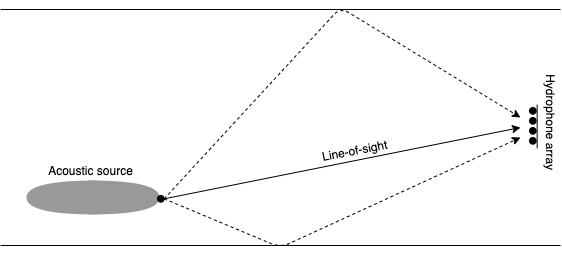
\includegraphics[width=0.8\textwidth]{figures/multipath}
	\caption{Illustrative example of shallow water multipath}
	\label{fig:mpath}
\end{figure}


\paragraph{Deep water paths} In deep water, there are essentially six types of propagation paths, detailed bellow, whose channel model equations can be consulted in \cite{multipath-rayleigh-models}. These rely on the notion that signals are bent towards the characteristics that lead to a slower propagation speed, such as a temperature and depth decrease.

\begin{itemize}
	\item \textit{Surface reflection}: the signal is reflected on the sea surface, where the attenuation depends on its acoustic roughness.
	
	\item \textit{Surface duct}: the signal gets confined in a surface layer, where the sound velocity increases with depth, due to varied thermal conditions in deeper layers, which causes it to bend the wave path to the surface and bounce back when reaching the subsequent layer.
	
	\item \textit{Bottom bounce}: the signal is reflected on the bottom of the ocean, suffering attenuation dependent on the soil material.
	
	\item \textit{Convergence zone}: it depends on the sound speed profile and water depth that characterizes the channel. When the temperature decreases the signal has a tendency to bent downwards, however when an increase in pressure is reached the signal tends to bent upwards again, originating convergence locations.
	
	\item \textit{Deep sound channel}: it is originated in levels that are surrounded by layers with characteristics highly dependent on depth. So, the signal is constantly bent according to the depth that leads to a minimum speed. 
	
	\item \textit{Reliable acoustic path}: this path occurs when the transmitter is positioned in very deep water and the receiver is near the surface. Although the signal is bent downwards due to decreased temperature, when it reaches a certain depth it is bent upwards making the communication channel reliable.
\end{itemize}

The multipath phenomena is a factor that commonly affects underwater communication mechanisms. The ray bending that occurs between the transmitter and the receiver can cause the signal to assume different paths and affect the resulting estimations. For instance, in positioning systems if the signal deviates from the direct path, then the angle of arrival would not be accurately perceived and the time of arrival increases, leading to an increased error on the range estimation.

\subsection{Doppler Effect} \label{subsec:doppler}

In a communication and localization system between two entities moving with non-zero relative velocity, if a transmitter sends a signal with a certain operation frequency to the receiver, then the perceived frequency by the receiver will suffer a shift from the original signal. This frequency difference is expressed as a Doppler shift and explained by the Doppler Effect.

The magnitude of the generated frequency shift can be expressed as a ratio (\ref{eq:ratio}), where the transmitter-receiver velocity is compared to \(c\), the speed of sound \cite{commchan}.

\begin{eqnarray}
&a = \frac{v}{c}
\label{eq:ratio}
\end{eqnarray}

Autonomous Underwater Vehicles (AUVs) usually move with velocities in the order of few meters per second. Therefore, the \(a\) factor mentioned above has a significant value and needs to be considered when implementing synchronization systems, as well as developing estimation algorithms.

In certain localization and communication systems, it is critical to correct the Doppler effect because data can be compromised (e.g. FSK modulated signals, in which information is codified into frequency changes). A simple Doppler compensation process was proposed in \cite{thesis-joao}, with the intent of integrating it in a system that detects phase-modulated binary sequences using cross-correlation.

This phenomenon can also be explored to determine the relative velocity between two devices, by measuring the frequency deviation with respect to the frequency expected to be received.

In applications such as underwater positioning systems, the Doppler effect can be a source of great measurement uncertainty. In USBL systems, the computation of the time difference of arrival depends on the perceived phase differences between the arriving signals, which are directly related to the operation frequency.  Therefore, a frequency shift would make the positioning system have a distorted perception of the phase differences and thus the signal's angle of arrival.

\subsection{Attenuation and Signal-to-Noise Ratio} \label{subsec:snr}

When considering underwater communication systems, it is essential to quantify the attenuation of the channel, i.e. the part of the signal's energy that is absorbed by the surroundings. In underwater channels, this absorbance is frequency variable and also depends on physical characteristics of the water, such as salinity and temperature. 

The underwater acoustic channel has a particular model that describes its attenuation path loss \(A(d,f)\) by equation (\ref{eq:attenuationdb}) \cite{pathloss}, given in logarithmic scale. 

\begin{eqnarray}
&10\ log(A(d,f)) = 10\ k\ log(d) + d \times 10\ log(a(f))
\label{eq:attenuationdb}
\end{eqnarray}

From the equation, \(d\) corresponds to the distance from the transmitter to the receiver in kilometers (Km), \(f\) is the operating frequency in kilohertz (KHz), \(10klog(d)\) represents the spreading loss that describes how the sound level decreases as the sound wave spreads in decibel, \(d \times 10 \ log(a(f))\) is the absorption loss that a signal suffers during its propagation path, \(k\) is the spreading factor that is related with the considered configuration (e.g. cylindrical, spherical, etc.), \(a(f)\) is the absorption coefficient that can be obtained through the equation (9) in \cite{pathloss}.

Noise is another factor that is considered when analyzing a real underwater acoustic channel, as it defines the signal-to-noise ratio (SNR) that characterizes the channel. The SNR depends on the attenuation level, which increases with frequency, and the noise, which decays with frequency. Consequently, the SNR varies over the signal bandwidth and it is asymmetric. Equation (\ref{eq:snr}) \cite{commchan} expresses this relationship, where \(S_{d}(f)\) represents the power spectral density of the transmitted signal.

\begin{eqnarray}
&SNR(d,f) = \frac{S_{d}(f)}{(A(d,f))\ N(f)}
\label{eq:snr}
\end{eqnarray}

Signals that are heavily attenuated can be an issue when dealing with acoustic positioning systems, such as USBL systems. If the transmitted signals suffer high attenuation then it may be unfeasible to rigorously detect the signal in the receiver, preventing the computation of the signal's angle of arrival or the transmitter's range. Additionally, in case of having a noisy environment it can be difficult to identify the intended acoustic signal, since it can be indistinguishable and blended with the noise. 

%________________________________________________________

\section{Underwater Localization}

Underwater localization is a key element in most underwater communication applications. An extensive survey on available algorithms and techniques is presented in \cite{und-localiz-survey}, highlighting their features, advantages, drawbacks and applications.

This section focuses on two types of underwater localization estimation techniques. Firstly, methods used for range estimation are presented, which include techniques based on the received signal's strength and on time delay estimation. Then, mechanisms for estimation-based localization are introduced, which include the two most used approaches, triangulation and lateration.

\subsection{Range Estimation}

Underwater localization takes into consideration the distance between the target object to track and the reference point. As consequence, it is relevant to apply methods that effectively determine this range.

There are two main types of techniques that are used to achieve such objective: the Received Signal Strength Indicator (RSSI) and the Time Delay Estimation (TDE).

\subsubsection{Received Signal Strength Indicator}

The Received Signal Strength Indicator (RSSI) method is based on the strength of the signal that reaches the target. It determines the distance between the target and the reference node by analyzing the received signal strength and comparing it with an underwater attenuation model that is range dependent \cite{ocean-acoust}.

Since the underwater acoustic channel suffers from multipath, time variance and high overall path loss, the RSSI technique is typically not adequate for long range underwater applications. However, in short range communications such effects can be sufficiently attenuated for this technique to be used.

\subsubsection{Time Delay Estimation}
Time Delay Estimation (TDE) mechanisms imply a pair of nodes, the transmitter and the receiver, to measure the range between them. This distance is based on the time that it takes for a signal to travel from the reference point to the target. The accuracy of these techniques depends mainly on the environment conditions, which include the water properties and the surrounding reflection surfaces that cause multipath. Therefore, the mechanisms are susceptible of variable errors according to the location and characteristics of its employment \cite{und-localiz-survey}.

There are three main categories that divide TDE methods, which are Time of Arrival (ToA), Time of Flight (ToF) and  Time Difference of Arrival (TDoA).

\paragraph{Time of Arrival}

Time of Arrival (ToA) is interpreted as the time delay between the transmission of a signal in the reference node until its reception on the receiver node. Although this is the conceptually simplest method to employ, it requires synchronization between the nodes since the receiver system needs to know the signal's time of emission to be able to calculate the total propagation time.

Considering a generic transmitted signal \textit{s(t)}, the received signal can be expressed as (\ref{eq:toa}), where $\tau$ represents the time of arrival and \textit{n(t)} is white noise with zero mean \cite{wirelesscomm}. 

\begin{eqnarray}
& r(t) = s(t - \tau) + n(t)
\label{eq:toa}
\end{eqnarray}

\paragraph{Time of Flight}

Time of Flight (ToF) measures essentially the round-trip travel time between two nodes \cite{und-localiz-survey}. The transmitter node sends a query signal to the receiver node, which has an integrated transponder that responds transmitting a signal back within a know time delay. The ToF is then estimated as the time interval from the moment the first signal is transmitted until the moment the second signal is received by the same node. 

This method may be used without additional synchronization systems as it assumes that the response signal is sent after the received one, with known intrinsic transmitting delays.

\paragraph{Time Difference of Arrival}

The Time Difference of Arrival (TDoA) is a technique that compares the time of arrival of a signal to different hydrophones in order to estimate the angle of arrival of the acoustic signal \cite{und-localiz-survey}. The array of reception hydrophones have known relative positions among them so that is is possible to compare the different times of arrival or phase differences. This method can be employed using a uni-directional signal or a round trip communication.

There are several algorithms and mathematical models that can be employed to execute the TDoA method, such as Cross-Correlation and Maximum Likelihood.

\begin{itemize}
	%----------------------------------------------------
	\item \textbf{Cross-Correlation}

The Cross-Correlation (CC) method  is used to represent the strength relationship between two signals. 

Considering two distanced hydrophones in the same environment and an acoustic signal \textit{s(t)}, \textit{$x_1$(t)} and \textit{$x_2$(t)} are the signals received by each of the two hydrophones. Equations (\ref{eq:gcc1}) and (\ref{eq:gcc2})\cite{crosscorr-76} express the mentioned signals in relation to \textit{$w_1$(t)} and \textit{$w_2$(t)} that are Gaussian noise coefficients uncorrelated with the source, the delay $\tau$ and an attenuation function $\alpha$.
\begin{eqnarray}
	&x_1(t) = s(t) + w_1(t)
	\label{eq:gcc1}\\
	&x_2(t) = \alpha \ s(t - \tau) + w_2(t)
	\label{eq:gcc2}
\end{eqnarray}

In order to determine the time delay, $\tau$, between signals, the cross-correlation function can be calculated as (\ref{eq:cc-def}). The estimate of the time delay between two signals, $\tau$, is given by $arg max_{\ t\in R^+} Rx_1x_2(\tau)$, which represents the maximum correlation value and it is the main outcome of Time Delay Estimation. 

\begin{eqnarray}
&R_{x_1x_2}(\tau) = E[x_1(t) \ x_2(t- \tau)]
\label{eq:cc-def}
\end{eqnarray}

However, since the observation time is finite then function $R_{x_1x_2}$ can only be estimated, originating equation (\ref{eq:cc-def-estim}) where $T$ expresses the observation interval.

\begin{eqnarray}
&\widehat R_{x_1x_2}(\tau) = \frac{1}{T - \tau} \ \mathlarger{\int_{\tau}^{T} x_1(t)x_2(t - \tau)} dt
\label{eq:cc-def-estim}
\end{eqnarray}
	
There are two main variations of CC \cite{crosscorr}, which are the slow cross-correlation in the  time domain, as before mentioned, and the fast cross-correlation in the frequency domain, which is based on the Fast Fourier Transform as it locates the peak by analyzing frequency similarities between the signals. 
	
	%----------------------------------------------------
	\item \textbf{Generalized Cross-Correlation}

After presenting the cross-correlation method, it is easier to understand the Generalized Cross-Correlation (GCC) method, which is extensively explained in \cite{crosscorr}. Recalling the equations that define the CC, the GCC is achieved by prefiltering the $x_1$ and $x_2$ prior to the integration in (\ref{eq:cc-def-estim}), using filters $H_1$ and $H_2$. Then the obtained filtered signals $y_1$ and $y_2$ are multiplied and integrated in a period of time $T$ until detecting the function peak.

Then the GCC between $x_1(t)$ and $x_2(t)$ is given by (\ref{eq:gcc3}), where the $G_{x_1x_2}(f)$ represents the cross power spectrum between the filter inputs. 

\begin{eqnarray}
	& R_{y_1y_2}(\tau) = \int_{-\infty}^{\infty} \psi(f) G_{x_1x_2}(f)\ e^{i2\pi f\tau} df
	\label{eq:gcc3}\\
	& \psi(f) = H_1(f)H_2^*(f)
	\label{eq:gcc4}	
\end{eqnarray}

The function $\psi(f)$ (\ref{eq:gcc4}), with $*$ denoting the complex conjugate, represents the prefilter and it is essentially the distinctive parameter that originate different methods of cross-correlation, since it should depend on different environments and properties, as SNR. The CC technique uses a prefilter $\psi(f)$ equal to 1, being the simplest method of its kind.

%----------------------------------------------------
\item \textbf{Maximum Likelihood}

The Maximum Likelihood (ML) method is a variation of Cross-Correlation which uses the prefilter $\psi(f)$ represented mathematically by (\ref{eq:ml1}), where $\gamma_{12}(f)$ is a function of spectrum of cross-correlation $G_{x1x2}(f)$ and spectrum of auto-correlations $G_{x1x1}(f)$, $G_{x2x2}(f)$ as expressed in (\ref{eq:ml2}) \cite{crosscorr}.

\begin{eqnarray}
& \psi(f) = \frac{|\gamma_{12}(f)|^2}{|G_{x1x2}(f)|[1-|\gamma_{12}(f)|^2]}
\label{eq:ml1} \\
& |\gamma_{12}(f)|^2 = \frac{|G_{x1x2}(f)|^2}{G_{x1x11}(f) . G_{x1x11}(f)]}
\label{eq:ml2} 
\end{eqnarray}

There is also a version of ML that uses the power spectral densities of the signals, which can be helpful for calculations in various applications. 
\end{itemize}

%________________________________________________________

\subsection{Estimation-Based Localization}

In networks with multiple nodes it is typical to use localization estimation to establish relative positions between elements. This is usually achieved by establishing reference nodes with known positions so that it is possible to determine relative positions based on them.

Two of the most commonly used methods for underwater acoustic positioning are Triangulation, which is based on the angles between nodes and the object to be located,  and Lateration, which is based on the range between the element to be located and each node \cite{triang-later}. These methods present two common restrictions: both need of a minimum of three visible nodes for 2D localization or four beacons for 3D localization and both fail to determine the unknown position if the nodes and the position to be estimated are all placed in the same circumference.

An extensive comparison of different localization schemes for underwater sensors networks can be consulted in \cite{suvey-loc}. 

\subsubsection{Triangulation}

Triangulation is a method widely used in mobile robot localization so various algorithms have been proposed. In \cite{class-triang}, triangulation methods are divided into four categories: 

\begin{itemize}
	\item \textbf{Geometric Triangulation}: comprises methods based on geometric relations and trigonometry;
	
	\item \textbf{Geometric Circle Interaction}: the algorithms calculate the radius and center of two circles that pass through the nodes and the object to be localized, so that the intersection between them gives the unknown localization;
		
	\item \textbf{Iterative methods}: includes algorithms that iteratively estimate the position by linearization of trigonometric relations;
	
	\item \textbf{Multiple Beacons Triangulation}: the methods use more than three angles to localize an object, which is usually used in scenarios with corrupted angle measurements.
\end{itemize}

Since this method was not adopted in the present dissertation, only a brief overview on the existing algorithms was made.

\subsubsection{Lateration} \label{subsubsec:lateration}

As mentioned before, lateration relies on the range between the object to be localized and multiple reference nodes. The most typically employed lateration technique is the multilateration, which is used in this dissertation. In this method, the employment of \textit{n+1} nodes allows to determine \textit{n} coordinates \cite{arch_localiz}. For instance, determining the position $(x,y,z)$ of an object requires to resolve a system of equations using (\ref{eq:mult}), where $(x_{i}, y_{i}, z_{i})$ are the coordinates of the node and $d_{i}$ is the distance between the node and the object.

\begin{eqnarray}
	& (x - x_{i})^2 + (y - y_{i})^2 + (z - z_{i})^2 = d_{i}^2 
	\label{eq:mult}
\end{eqnarray}

Figure \ref{fig:trilateration} illustrates a specific case of trilateration, which implies the use of three reference nodes 1, 2 and 3. The object $O$ corresponds to the position to be localized that is determined by calculating the intersection between the three circumferences, generated by knowing the relative positions and ranges, $d_1$, $d_2$ and $d_3$, between all elements.

\begin{figure}[!htbp]
	\centering
	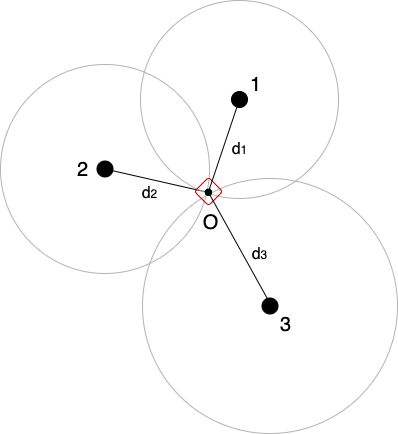
\includegraphics[width=0.5\textwidth]{figures/trilateration}
	\caption{Localization using trilateration}
	\label{fig:trilateration}
\end{figure}

Distributed mechanisms, such as multilateration, are usually divided in three phases of positioning \cite{suvey-loc}:
\begin{itemize}
	\item Distance estimation between the reference nodes and the target object, usually using TDoA or ToF mechanisms;
	\item Position estimation, obtained by solving a system of linear equations through mathematical techniques or sensor fusion using an estimator, since the solutions are usually approximated due to noise or non-linearities;
	\item Final refinement of the measurement in order to improve accuracy.
\end{itemize}

As an alternative to solve localization issues using circumferences, multilateration can also take advantage of a hyperbola-based localization method. Considering a target at (x,y) and three reference beacon with coordinates $(x_{i},y_{i})$,  $(x_{j},y_{j})$ and  $(x_{k},y_{k})$, we have that the difference between times of arrival $t_{i}$ and $t_{j}$ to nodes $i$ and $j$, respectively, can be related to the distance between nodes, as expressed in (\ref{eq:hyper}) \cite{arch_localiz}. $d_{i}$ and $d_{j}$ are the distance from node $i$ and $j$, respectively, to the target object. 

\begin{eqnarray}
	& d_{i} - d_{j} = c * (t_{i} - t_{j}) = \sqrt{(x - x{i})^2 + y - y{i})^2} - \sqrt{(x - x{k})^2 + y - y{k})^2}
	\label{eq:hyper}
\end{eqnarray}

%________________________________________________________

\section{Underwater Acoustic Positioning Systems}

Positioning systems are used to track the underwater position of a vehicle or other object, in relation to reference structures of transponders called \textit{baseline stations}. These systems are classified based on the distance between the baseline stations. The configurations that will be explained are Long Baseline (LBL), Short Baseline (SBL), Ultra-Short Baseline (USBL) and the inverted versions of all above.

\begin{figure}[!htbp]
	\centering
	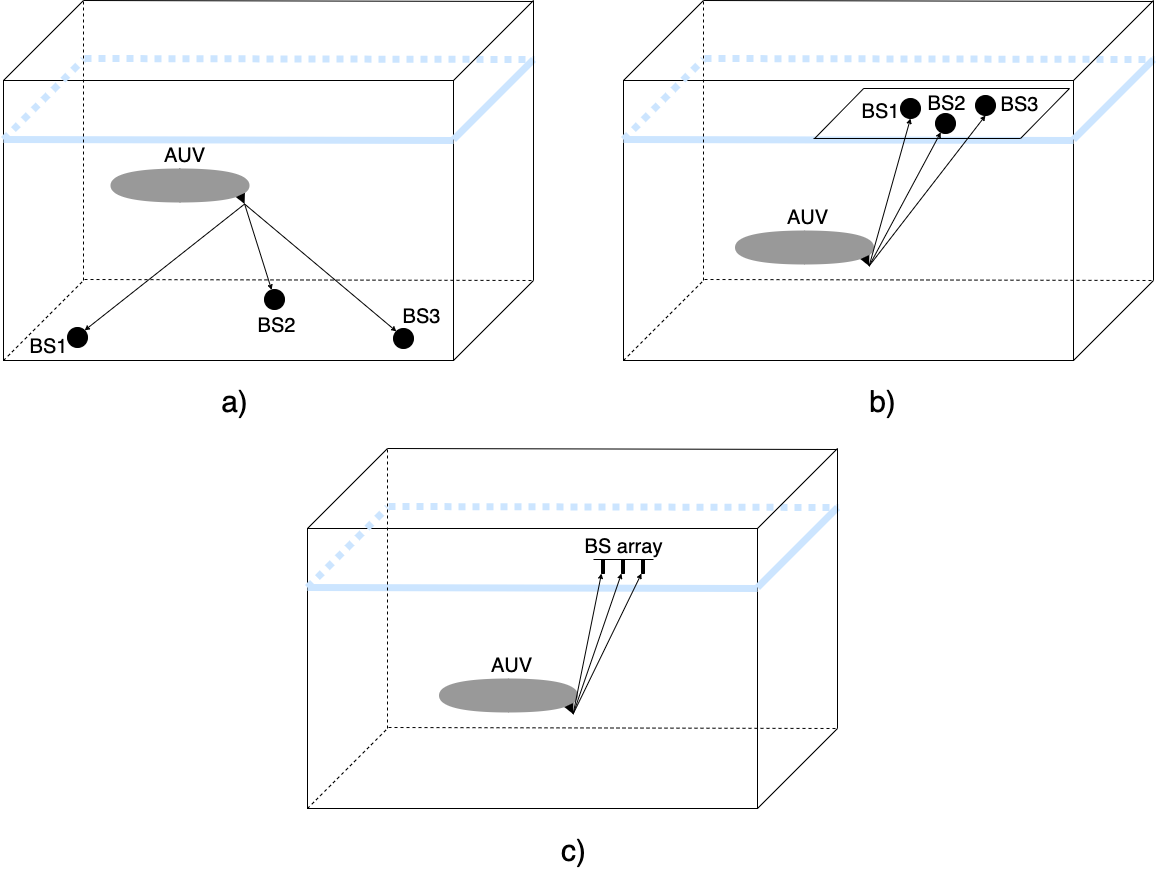
\includegraphics[width=1\textwidth]{figures/lblsblusbl}
	\caption{Generic configuration of: a) LBL; b) SBL; c) USBL}
	\label{fig:lblsblusbl}
\end{figure}

\subsection{Long Baseline (LBL) and Short Baseline (SBL)}

Long Baseline (LBL) and Short Baseline (SBL) systems are characterized by different ranges and transponder deployment, however they share the same operating procedure.

Long Baseline systems use a positioning method with large distances between baseline stations, with a range typically from $50m$ to more than $2000m$ and usually similar to the distance between the receiver and the transponders \cite{crosscorr}. A typical LBL configuration is represented in illustration a) of \ref{fig:lblsblusbl}. It uses at least three transponder stations deployed usually on the sea floor.

Short Baseline systems are characterized by having distances around $20m$ to $50m$ between baseline stations \cite{survey-tech-chall} and uses transponders usually placed in a moving platform, assuring fixed relative position between them. A typical SBL configuration is represented in illustration b) of \ref{fig:lblsblusbl} \cite{leassquare-lbl}.

For both LBL and SBL, a complete localization procedure starts with the vehicle sending an acoustic signal which is received by the transponders. Thereafter the transponders transmit a response and, by analyzing the Time of Flight of the communication,it is possible to determine the distance between the vehicle and each transponder. Then the relative position of the vehicle is determined through trilateration. Considering $t_{i}$ the propagation time of the signal from the vehicle to the \textit{i}th transponder, $c_s$ the speed of sound and ($x_{b_{i}}$, $y_{b_{i}}$, $z_{b_{i}}$) as the coordinate position of the transponder, then equation (\ref{eq:sbl}) \cite{sbl} expresses the position of the vehicle. Additionally, if the transponders have known geographic positions, it is possible to infer the vehicle's absolute geographic position. 

\begin{eqnarray}
	&\sqrt{ (x_{b_{i}}-x)^2 + (y_{b_{i}}-y)^2 + (z_{b_{i}}-z)^2 } = c_s\ *\ t_{i}
	\label{eq:sbl}
\end{eqnarray}


The accuracy of these methods depend on several factors, such as the range of communication and transponders configuration, and it typically fluctuates between tens of centimeters and a few meters.


\subsection{Ultra-Short Baseline (USBL)}

Ultra-short Baseline systems are composed essentially by one baseline station, with an array consisting of several traducers distanced typically less than the wavelength \cite{lblsblusbl}, and a transponder integrated on the vehicle. It is usually represented as illustration c) of \ref{fig:lblsblusbl}.

Similarly to the previously mentioned procedures, the USBL positioning method relies on the Time of Flight of the exchanged signals. However, the traducers are too spatially close from each other to execute an accurate trilateration. Instead, it is measured the phase difference or time-delay difference of the received signal between every traducer, in order to estimate the azimuth and distance to the acoustic source. 

Assuming a three dimensional scenario for the positioning system, as represented in figure \ref{fig:usblgeo}, the object's coordinates are given by equations (\ref{eq:usblgeo1}), (\ref{eq:usblgeo2}) and (\ref{eq:usblgeo3}) \cite{usbl-new}. The $\lambda$ corresponds to the wavelength of the of the transmitted signal which depends on its operation frequency, \textit{f}, and it is affected by the speed of sound \textit{c}, as represented equation (\ref{eq:cfw}).
The \textit{d} represents the distance between hydrophones, $\psi_{12}$ and $\psi_{22}$ are the phase difference between H2 and the other two hydrophones, \textit{H} is the height of the target object, \textit{X} is the distance of the target along the x-axis direction, \textit{Y} is the distance of the target along the y-axis direction and \textit{l} is the slant distance of the target to the hydrophone.
\begin{eqnarray}
& \lambda = \frac{c}{f}
\label{eq:cfw}
\end{eqnarray}
\begin{eqnarray}
& l^2 = X^2 + Y^2 + H^2 
\label{eq:usblgeo1}\\
& \psi_{12} = \frac{2\pi}{\lambda}[\sqrt{l^2} - \sqrt{(d-X)^2 + d^2 + H^2}]
\label{eq:usblgeo2}\\
& \psi_{22} = \frac{2\pi}{\lambda}[\sqrt{l^2} - \sqrt{X^2 + (d-Y)^2 + H^2}]
\label{eq:usblgeo3}
\end{eqnarray}

\begin{figure}[!htbp]
	\centering
	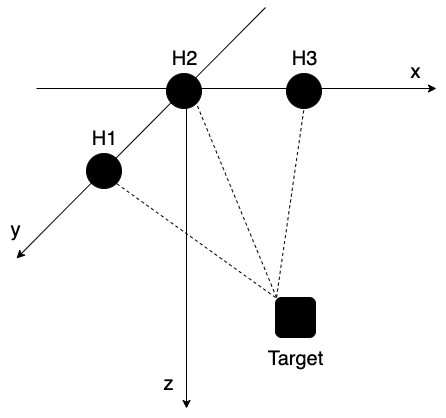
\includegraphics[width=0.5\textwidth]{figures/usbl-config}
	\caption{USBL system configuration}
	\label{fig:usblgeo}
\end{figure}

This is a broadly used technique due to its convenient set up, which allows to have predefined measurements in the order of tens of centimeters and does not require the deployment of support infrastructures in the intended navigation area of the target AUV. However, since the USBL is based on bearing determination it needs high accuracy in order to achieve efficient localization estimations.. 


%\subsection{Inverted Systems}
%
%All the previously mentioned positioning techniques use a configuration in which the vehicle to be tracked has a single transducer and there is an external set of transponder to determine the positioning of the said object. However, there is the possibility to benefit from the inverse configuration in some applications. Therefore, there are also the iLBL, iSBL and iUSBL methods, which have the same operation principals as LBL, SBL and USBL, respectively.

%_________________________________________________________


\section{Commercial Solutions}

There are several commercial solutions for underwater positioning using the Ultra-Short Baseline method. In this section, some of the available devices in the market will be presented, indicating their main properties and capabilities. Table \ref{tab:solutions} summarizes the systems with most relevance to the present work in terms of used bandwidth, connection link, maximum range and precision. The Medium Frequency (MF) bandwidth is attributed to devices whose manufacturer did not specified the actual frequency range. The specified precision depends on the available information, which varies between slant range precision (SR) and range detection (RD).

\textit{Evologics} produces the S2C R USBL series of acoustic modems \cite{evologics1}, with Sweep Spread Carrier (S2C) technology \cite{evologics2} which uses a broad frequency range to propagate over large distances with reduced noise. The devices have a fixed 0.01m slant range precision and a 0.1 degree bearing resolution. These are essentially divided into two groups:
\begin{itemize}
	\item High speed mid-range devices: contains the 18/34 transceivers family \cite{evologics3}, which presents various options for the USBL antenna beam pattern and it is designed for transmission in horizontal channels.
	\item Depth rated long-range devices: includes the 12/24 transceiver \cite{evologics4}, which have a directional (70 degrees) USBL antenna  and it is designed for transmission in vertical channels.
\end{itemize}

\textit{Sonardyne} markets the Ranger 2 systems. The Micro-Ranger 2 \cite{sonardyne1} is appropriate for shallow waters, achieving accuracy of 0.2\% with a $3Hz$ position update rate. The Mini-Ranger 2 \cite{sonardyne2} is intended for nearshore missions and it is  used for simultaneous tracking of various mobile targets, whose position update rate is $3Hz$ as well.

\textit{Applied Acoustics} offers the Easytrak USBL Systems \cite{applied-easytrak}, which includes the processing software for estimating the position. The Alpha Portable 2655 consists in a very compact structure that includes an array transducer and is capable of reaching a 10cm slant range resolution and a 2 degree RMS.

\textit{Kongsberg} produces the HiPAP family of transducers \cite{hipap_hardw}, which can use the Cymbal acoustic protocol (PSK) or the frequency shift (FSK) modulation technique. Particularly the HiPAP 352 is the model with higher number of active transducers and is able to reaches 0.02m of range precision.

\begin{table}[!htbp] %use !htbp to adjust
	\begin{center}
	\makebox[\textwidth]{
	\begin{tabular}{l|l l l l l}
		\toprule
		\textbf{Company} & 
		\textbf{System} & 
	   \begin{tabular}{@{}l@{}}\textbf{Bandwidth} \\ \textbf{(kHz)}\end{tabular}&
		\begin{tabular}{@{}l@{}}\textbf{Connection} \\ \textbf{(kbps)}\end{tabular}&
		\begin{tabular}{@{}l@{}}\textbf{Max Range} \\ \textbf{(m)}\end{tabular} &
		 \begin{tabular}{@{}l@{}}\textbf{Precision} \\ \textbf{}\end{tabular} \\ 
		\midrule
		\multirow{2}{4em}{Evologics} 
		& S2C R 18/34D USBL & 18-34 & up to 13.9 & 3500 & 0.01m (RD) \\
		& S2C R 12/24 USBL & 12-24 & up to 9.2 & 6000 & 0.01m (RD)\\
		\midrule 
		\multirow{2}{4em}{Sonardyne} 
		& Micro-Ranger 2 & MF & 0.2-9 & 995 & 5\% (SR) \\
		& Mini-Ranger 2 & MF & 0.2-9 & 995 & 1.3\% (SR) \\ 
		\midrule 
		\begin{tabular}{@{}c@{}}Applied \\ Acoustics\end{tabular}
		& Easytrak Alpha Portable 2655 & MF & n.d. & 500 & 3.5\% (SR)\\
		\midrule 
		\multirow{1}{4em}{Kongsberg} 
		& HiPAP 352 & 21-31 & n.d. & 5000 & $0.02m$ (RD) \\
		\bottomrule 
	\end{tabular}}
	\caption{Overview of commercial solutions}
	\label{tab:solutions}
	\end{center}
\end{table}

% http://www.teledynemarine.com/usbl-dat?ProductLineID=59
% https://www.link-quest.com/html/tl10000.pdf
% https://www.tritech.co.uk/product/usbl-tracking-system-micronnav
%_______________________________________________________________________________


\section{Optimization of Sensor Configurations}

When dealing with positioning systems, such as USBL, it is necessary to deploy sensors in the vehicle that is intended to locate a transmitter emitting acoustic signals. Therefore, it is considered that four hydrophones are needed to measure the time difference of arrival of a received acoustic signal so its direction can be calculated. These hydrophones can be located anywhere along the boy of a vehicle, so it is essential to understand how can the sensor layout be designed, namely in terms of its physical distribution along the body of an underwater structure, in order to achieve the best possible estimation. 

This section is dedicated to explore some commonly employed methodologies which evaluate the performance of sensor layouts considering determined parameters. Firstly, the Crámer-Rao Lower Bound and the Fisher Information Matrix are presented, followed by the optimality criteria for design optimization. Lastly, the Particle Swarm Optimization is presented as a widely used method that uses artificial intelligence concepts to achieve an optimal design.

\subsection{Crámer-Rao Lower Bound}	\label{sec:cramer}

The Crámer-Rao lower bound (CRLB) is a tool which analyzes the variance of a sensor configuration and determines the minimum bound it can achieve independently from the used estimator. This method assumes the usage of an efficient estimator, which is an optimal estimator for the chosen parameter, and an unbiased estimator, i.e. the real value of the parameter which is equal to the expected value.

In this thesis, it is conducted a study based on the CRLB, which is generally used to generate a \textit{so-called uncertainty ellipse} \cite{bishop-cramer-rao} that represents the spatial distribution or the spatial variance distribution of the estimated position. The overall desired result is to find the minimum variance that is related to the chosen configuration geometry, which indicates that it is the optimal solution for estimating a certain position. This method utilizes the Fisher Information matrix (FIM) as explained next, which measures the quantity of information that can be extracted from an observation vector about a certain parameter.

In order to avoid loss of generality, it is considered a set of N sensors and a settled position for the acoustic source, defined by $s$ = [$x_{s}$, $y_{s}$, $z_{s}$]$^T$. In addition, the position of each sensor is defined as $r_{i}$ = [$x_{r_{i}}$, $y_{r_{i}}$, $z_{r_{i}}$] and, consequently, the measurement of distance between each sensor and the source is defined as d$_{i}$ = $|| s - r_{i} ||$.

Thereafter, the observations vector will be formulated containing the observed times-of-arrival (ToA) of the signal from the acoustic source to each one of the hydrophones, considering their geometric position. These times contain a noise vector component, which can be approximated to a Gaussian distribution $n_i \sim \mathcal{N}(\mu,\,\sigma^{2})$. The samples can be calculated through the expression (\ref{eq:obs_vec}), where it is considered an initial time of emission $t_0$. Additionally, c represents the sound speed underwater.

\begin{eqnarray}
	t_i = t_0 + \frac{||d_i||}{c} + n_i
	\label{eq:obs_vec}
\end{eqnarray}

After having the observations matrix, the condition to formulate the Fisher Information matrix, $I(d)$ , is established which results into equation \ref{eq:fisher}.

\begin{eqnarray}
	I(d) = \nabla_{d}t(d)^T \; \Sigma^{-1} \; \nabla_{d}t(d)
	\label{eq:fisher}
\end{eqnarray}

$\nabla_{d}t(d)$ is the gradient matrix of the observations vector regarding $d_i$, whereas $\Sigma$ is the covariance matrix, in which the diagonal contains the standard deviation of the components of each noise vector, construed as $(\sigma_1^2 , \sigma_2^2 , ... , \sigma_N^2)$ .

The Fisher Information Matrix quantifies the information that a certain sensor configuration can give about a position in space. Hence the goal is to obtain the maximum achievable information. By calculating the determinant of FIM it is possible to deduce the minimum \textit{uncertainty ellipsoid} and therefore the configuration's best possible performance. Therefore, the optimal solution is given by the maximum output of the determinant of FIM.

Additionally, it is possible to detail this information by calculating the actual size of the axis that compose the \textit{uncertainty ellipsoid}. This is achieved by calculating the square mean root of the eigenvalues of $I(d)$, which correspond to each axis size.

Therefore, the Crámer-Rao lower bound is widely used as a metric to evaluate the performance of sensor configurations. Further explanation about the methods used in a deeper exploration of the Crámer-Rao lower bound can be consulted in \cite{bishop-cramer-rao}. However, the mentioned concepts were all the necessary for the approach on this dissertation .

This same process is adopted in this dissertation. All steps specifically taken for this study are declared in section \ref{sucsec:FIM} of the present document.

%_______________________________________________________________________________
%_______________________________________________________________________________

\subsection{Optimal Design and Optimality Criteria}	\label{sec:optimaldesign}

When contemplating system designs, the optimal solution for a problem is generally a subjective matter which depends on the chosen criterion. Following this idea, we can define optimal designs as experimentally generated designs of various types of systems which are usually optimal for a targeted statistical model and are modeled by a specific optimality criterion. These criteria can be organized in four distinct groups \cite{compare-optimality-crit}:
\begin{itemize}
	\item \textbf{Information-based} : comprehends all criteria that are related to the Fisher information matrix $X'X$. Some of the criteria which fits into this category are A-, D-, E- and G-optimality.
	\item \textbf{Distance-based} : includes criteria which depends on the distance $d(x,A)$ from a point $x$ in the Euclidean space $\mathbb{R}^{p}$ to a set $A \subset \mathbb{R}^{p}$. U and S-optimality are integrated in this category.
	\item \textbf{Compound design} : combine different adjusted criteria in different weighted proportions in order to meet a desired statistical function.
	\item Other : all criteria which do not fit in the previous three sets can be encompassed in a fourth general set.
\end{itemize}

The most relevant category for the present work is the information-based criteria, since we want to maximize the information that can be extracted from a certain design and we do not need to minimize the distances between the receptors and the source. Therefore some of the most commonly used criteria will be better explained in the following subsections, which correspond to the chosen metrics for optimizing the localization precision during the present research work.

\subsubsection{A-optimality}

The A-optimality criterion intends to minimize the trace of the inverse FIM, i.e. the mean-squared error (MSE) \cite{d-opt-mislead}. This corresponds to minimizing the summed eigenvalues of the FIM, which correspond to the length of the uncertainty axis, denoted as (\ref{eq:-a-opt-trace}).

\begin{eqnarray}
	& min( \ trace(I^{-1}))
	\label{eq:-a-opt-trace}
\end{eqnarray}

%\begin{eqnarray}
%&	I = 
%	\begin{bmatrix}
%		\psi_{11} & \psi_{12} & \psi_{13} \\
%		\psi_{21} & \psi_{22} & \psi_{23} \\
%		\psi_{31} & \psi_{32} & \psi_{33} 
%	\end{bmatrix}
%\label{eq:fisher-a-opt}\\
%&tr(CRLB) = tr(I ^{-1}) \geq \frac{1}{\psi_{11}} + \frac{1}{\psi_{22}} + \frac{1}{\psi_{33}} 
%\label{eq:-a-opt-trace}
%\end{eqnarray}

In applications where it is desirable to achieve a balanced uncertainty estimation in all directions, the A-optimality can lead to misleading conclusions as it can disguise larger uncertainty magnitudes in a single direction.

\subsubsection{D-optimality}

The D-optimality criterion minimizes the volume of the uncertainty ellipsoid associated with a specific estimate \cite{d-opt}. This is achieved by maximizing the FIM determinant, which maximizes the information that is possible to be obtained for a specific estimation. Alternatively, it can also be described as intending to minimize the determinant of the inverse FIM, (\ref{eq:d-opt-eq}), which corresponds to minimizing the ellipsoid uncertainty volume. This metric is widely used to achieve an optimal sensor geometry for single target estimation and 2D sensor placement. 

\begin{eqnarray}
	& min( \ det(I^{-1}))
	\label{eq:d-opt-eq}
\end{eqnarray}

This criterion presents advantages comparatively to other criteria, namely it is invariant under parameter scale changes and linear transformations of the output However, this optimization criteria can be misleading since a determinant value that is minimal can be disguising an ellipsoid uncertainty axis that is much larger than the remaining for the same estimate \cite{d-opt-mislead}, leading to a disproportionate estimation precision that it intended to be avoided.


\subsubsection{E-optimality}

The E-optimality criterion intends to minimize the maximum eigenvalue of the inverse FIM, i.e. minimizes the larger ellipsoid uncertainty axis corresponding to direction with the worse estimation precision. Expression (\ref{eq:e-opt-eq}) \cite{compare-optimality-crit} denotes this condition, where $\lambda_{max}$ is the maximum eigenvalue of the inverse FIM.

\begin{eqnarray}
	& \lambda_{max}(I^{-1})
	\label{eq:e-opt-eq}
\end{eqnarray}

Although this criteria is mitigating the worse ellipsoid uncertainty direction, it does not take into account the entirety of the ellipsoid uncertainty volume. It is usually the preferred criteria in applications where it is necessary to have a more homogeneous estimation precision in all directions, such as for approximation of objects that should not collide. 

As the present dissertation considers a scenario that requires the approximation of AUVs, which would to be preferably placed within few centimeters from each other, the E-optimality is considered the most relevant throughout the results analysis of this research work.

\subsection{Particle Swarm Optimization}

The Particle Swarm Optimization (PSO) is a Swarm Intelligence based computational method, which iteratively improves the candidate to a solution of a problem through cost functions. It is based on the behavior of environment entities (particles), such as fish schools or flocks of birds, and it approximates a candidate to the optimal solution by moving each particle in the direction of its previously best position ($pbest$) and the global best position ($gbest$) \cite{pso-surv}.

Given the standard algorithm for the PSO, equation (\ref{eq:pso-1}) expresses the velocity $V_i$ of the particles movement, which can be limited to avoid that particles fall of the intended region, and (\ref{eq:pso-2}) is the position $P$ that is updated. Additionally, the $t$ corresponds to the current iteration number, $i$ is the particle index, $w$ denotes a inertia weight that balances the global and local exploration, $c_1$ and  $c_2$ are acceleration coefficients and $r_1$ and  $r_2$ are random variables uniformly distributed withing the range [0,1].

\begin{eqnarray}
& V_i(t+1) = w V_i(t) + c_1 r_1 (pbest(i,t) - P_i(t)) + c_2 r_2 (gbest(t) - P_i(t))
\label{eq:pso-1}\\
& P_i(t+1) = P_i(t) + V_i(t+1)
\label{eq:pso-2}
\end{eqnarray}

A comprehensive survey on PSO algorithm adaptations and common applications is presented in \cite{pso-surv}, which include optimization of sensor localization for estimation improvement. 

In this regard, article \cite{particle-swarm-opt} explores the use of PSO to determine an optimal receiver configuration for Short-Baseline localization, which corresponds to a similar application to the conducted research in the present dissertation. In this study, a single transducer is placed on an AUV and four receivers are mounted on a mothership. The position estimation is based on the Euclidean distances between the transmitter and the receivers. After applying the PSO it is concluded that the optimal configuration achieved is different than the initially expected, leading to a 6.64\% improvement on estimation precision.
